\newpage
\clearpage

\section{Desenvolvimento do Projeto}
\label{project:project}

\subsection{Materiais e Métodos}
\label{project:matmet}
Nesta Seção, serão discorridos os detalhes sobre as tecnologias que serão utilizadas para o desenvolvimento de um modelo de segmentação panóptica que segmenta componentes visuais (Seção \ref{project:tec}), as técnicas e métodos escolhidos para serem utilizados nos experimentos (Seção \ref{project:method}) e, por fim, sobre os conjuntos de dados selecionados para cumprirem com o objetivo da segmentação (Seção \ref{project:dataset}).


\subsubsection{Tecnologias}
\label{project:tec}
Dentre as tecnologias planejadas para o desenvolvimento do presente trabalho, vale citar que destaca-se o uso da linguagem de programação interpretada e de alto nível, \textit{Python}, sendo essa uma linguagem vantajosa por ser popularmente conhecida no meio cientifico, com uma ampla comunidade e com  bibliotecas dispostas para facilitar o desenvolvimento de soluções \cite{Millman2011PythonEngineers}.

Já em relação às bibliotecas planejadas ao projeto, destacam-se aquelas cujo desenvolvimento é amplamente utilizado para o auxilio de projetos de visão computacional, aprendizado de máquina e redes neurais, das quais cita-se: \textit{PyTorch}, \textit{Keras}, \textit{TensorFlow}, \textit{OpenCV}, \textit{Numpy}, \textit{Pandas}, entre outras, dando destaque para a biblioteca \textit{Detectron2} \cite{detectron2} que já possui algumas funções especializadas para o trabalho com segmentações, incluindo redes de segmentação panóptica.

Por fim, em relação aos métodos desenvolvidos para cumprir com os objetivos do presente trabalho, no que lhes concerne, de realizar a segmentação de componentes visuais, declara-se que serão disponibilizado em forma de biblioteca por meio do \textit{Github} do autor\footnote{Perfil \textit{Github} do autor – \url{https://github.com/Lucs1590}}, segundo os preceitos a licença Apache v2.0 \cite{Licenses}, com o intuito de contribuir com o crescimento de futuros pesquisadores, além de possibilitar futuras melhorias da aréa de segmentação com uso de segmentação hierárquica.


\subsubsection{Métodos}
\label{project:method}
Dentre os métodos disponíveis para realizar a tarefa de segmentação panóptica de componentes visuais, destaca-se que serão realizados testes a partir dos modelos disponibilizados pela biblioteca \textit{Detectron2} \cite{detectron2}, seguindo também a formatação inicial proposta por Kirillov \textit{et al.} \cite{Kirillov2019a}, a qual era composta por um modelo de Mask R-CNN (Seção \ref{instance:mask}) para realizar a parte de segmentação de instâncias e o modelo de FCN (Seção \ref{semantic:FCN}) para realizar a segmentação semântica.

Todavia, haja vista o resultado esperado nesse trabalho, vide a Seção \ref{project:expres}, para as tarefas de segmentação panóptica com o uso de partes, diferente das abordagens de estruturas que possuem apenas as tarefas de segmentações de instâncias e semântica, seja de modo compartilhado, unificado, com conexões ou cascata, como demonstradas na Figura \ref{project:method:fig:1}, a segmentação de partes cientes necessita, também, de uma parte voltada para a segmentação das partes de objetos classificados como \textit{thing} ou \textit{stuff}, como demonstrado na Figura \ref{project:method:fig:2}, a qual representa uma estrutura voltada para a segmentação panóptica de modo unificado (segmentação semântica e de instância) e outra para a segmentação de partes cientes. Sendo assim, também será testada a estrutura desenhada por de Geus \textit{et al.} \cite{DeGeus2021}, a qual é composta por um modelo de segmentação panóptica (DLv3-ResNeSt269 \& DetectoRS) juntamente com um modelo responsável por realizar uma segmentação de partes (BSANet).

\begin{figure}[H]
    \centering
    \caption{Metodologias de rede para segmentação panóptica.}
    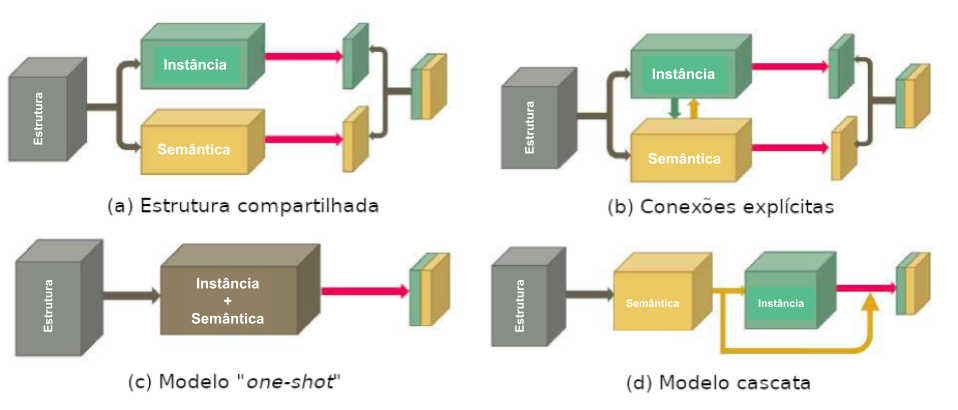
\includegraphics[width=1\textwidth]{recursos/imagens/proposal/model_methodologies.png}
    \label{project:method:fig:1}

    Fonte: retirado e adaptado de \cite{Elharrouss2021}.
\end{figure}

\begin{figure}[H]
    \centering
    \caption{Estrutura exemplificando metodologia para segmentação \textit{Part-Aware}.}
    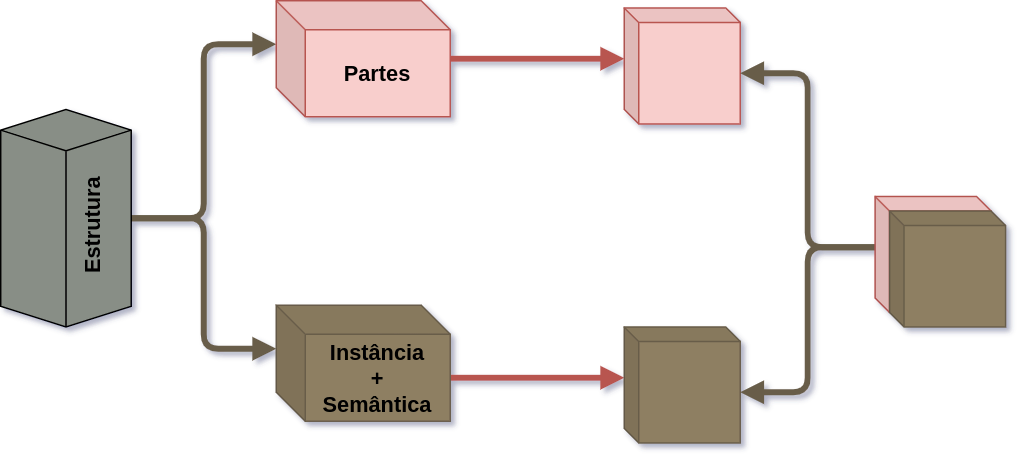
\includegraphics[width=4in]{recursos/imagens/proposal/estrutura.png}
    \label{project:method:fig:2}

    Fonte: do próprio autor.
\end{figure}



\subsubsection{Anotação de Dados}
\label{project:annotation}



\subsubsection{Conjuntos de Dados}
\label{project:dataset}
Em relação ao conjunto de dados, por esse trabalho fazer uso da segmentação \textit{Part-Aware Panoptic Segmentation} proposta em \cite{DeGeus2021}, sendo que esta é uma nova abordagem, vale dizer que a quantidade de conjuntos de dados ainda é escassa, principalmente quando se trata de trabalhos voltados para uma área em específico, como a odontológica.

Todavia, no presente trabalho serão utilizados tanto conjuntos de dados que são mais generalistas, mas são voltados para a segmentação panóptica, quanto conjuntos de dados voltados para a parte odontológica, os quais precisarão ser anotados de modo a estarem adaptados para o seu uso em bases de treino e teste.

Quanto aos conjuntos de dados mais generalistas vale dizer que há algumas estratégias e justificativas para o seu uso, as quais serão descritas na Seção \ref{project:transf}, entretanto, dentre os conjuntos de dados escolhidos, destacam-se PASCAL \textit{Panoptic Parts} e \textit{Cityscapes Panoptic Parts}, sendo que os estes foram desenvolvidos pelos autores que abrolharam a segmentação panóptica com uso da técnica \textit{Part-Aware} \cite{DeGeus2021}.

O conteúdo dos conjuntos PASCAL \textit{Panoptic Parts} e \textit{Cityscapes Panoptic Parts} foram criados a partir dos conjuntos de dados \cite{everingham2010pascal} e \cite{Cordts2016}, sendo que o conteúdo do primeiro está voltado para pessoas, animais, veículos e cenas em locais fechados, quando o segundo conta com cenas de cidades, respectivamente, os quais são exemplificados na Figura \ref{project:dataset:fig:1}.

\begin{figure}[H]
   \caption{Imagens originais e anotadas dos \textit{datasets} para \textit{Part-Aware Panoptic Segmentation}.}
   \centering
   \label{project:dataset:fig:1}
    \begin{subfigure}[t]{0.45\textwidth}
        \centering
        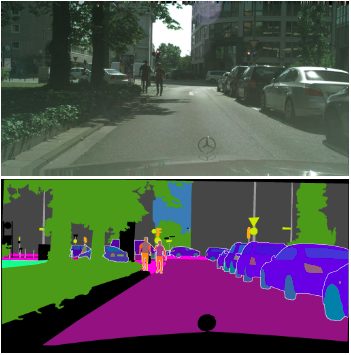
\includegraphics[height=2.5in]{recursos/imagens/proposal/city.png}
        \caption{Imagem original e anotada do \textit{Cityscapes Panoptic Parts}, respectivamente.}
        \label{project:dataset:fig:1.1}
    \end{subfigure}%
    ~ 
    \begin{subfigure}[t]{0.45\textwidth}
        \centering
        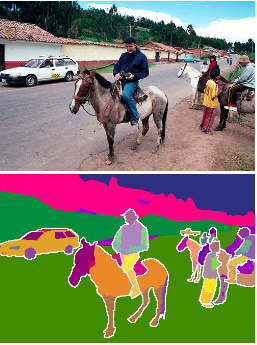
\includegraphics[height=2.5in]{recursos/imagens/proposal/pascal.png}
        \caption{Imagem original e anotada do PASCAL \textit{Panoptic Parts}, respectivamente.}
        \label{project:dataset:fig:1.2}
    \end{subfigure}%

    Fonte: retirado e adaptado de \cite{Lin2016}.
\end{figure}


Os conjuntos criados por \cite{DeGeus2021}, os quais contemplam segmentação \textit{Part-Aware}, quando relacionado ao \textit{Cityscape Panoptic Parts}, vale dizer que este possui 2975 imagens para treino e 500 para validação, totalizando em 3475 imagens dispostas em resolução de 1024×2048. Por sua vez, o PASCAL \textit{Panoptic Parts} possui 4998 imagens para treino e  5105 imagens para validação, as quais estão em resoluções de 387×470, totalizando à disposição de 10103 imagens.

Por fim, ainda há a disposição do conjunto de dados de partes, do qual se cita \textit{PartNet} \cite{mo2019} e \textit{PartImageNet} \cite{He2021}, sendo que o primeiro abrange a anotação de 573585 partes de instâncias, realizando a cobertura de 24 categorias de objetos, as quais também podem ser úteis para agregar ao projeto. Já o segundo, por ter sido criado com base no trabalho desenvolvido por \cite{DeGeus2021}, encontra-se disponível para o exercício das redes panópticas \textit{part-aware}, com 158 classes e por volta de 24000 imagens, visto que a fonte das imagens anotadas é o projeto \textit{ImageNet}.

Quanto aos conjuntos de dados comentados anteriormente que estarão dispostos para o meio odontológico, vale citar que esses não possuem uma anotação com classes de partes, as quais se fazem \textit{mister} para a aplicação panóptica com uso de \textit{Part-Aware}, todavia vale destacar que temos uma parceria da Faculdade de Odontologia de Araraquara (FOAr) - UNESP, a qual terá com líder o Prof. Dr. Osmir Batista de Oliveira Júnior, de modo que estudantes e especialistas da área realizem as anotações, bem como a disponibilização, de 5000 imagens de fotografias odontológicas, de modo a contribuírem para o projeto.

Além das fotografias cedidas pela parceria, vale destacar que alguns conjuntos de dados serão utilizados com o intuito de agregar em volume de imagens odontológicas, dos quais, cita-se o conjunto de dados desenvolvido por You \textit{et al.} \cite{You2020}, o qual possui 886 anotadas, o conjunto desenvolvido por Hyttinen \textit{et al.} \cite{Hyttinen2020}, com 316 imagens, sendo que 215 dessas imagens possuem uma anotação inicial e, por fim, o conjunto de dados disponível no \textit{website} da \textit{Dental Care}\footnote{\textit{Website \textit{Dental Care}} – \url{https://www.dentalcare.com/en-us/research/media-library}}, o qual cede 839 imagens odontológicas como cortesia para estudos e desenvolvimento científico. O objetivo é que todas essas 1370 imagens sejam agregadas à \textit{pipeline} de anotação e ao conjunto disponibilizado pela parceria, de modo a se tornarem úteis para a construção do modelo proposto no presente trabalho. Exemplos dos conjuntos de dados citados podem ser observados na Figura \ref{project:dataset:fig:2}.

\begin{figure}[H]
    \centering
    \caption{Exemplo de imagens dos conjuntos de dados odontológicos.}
    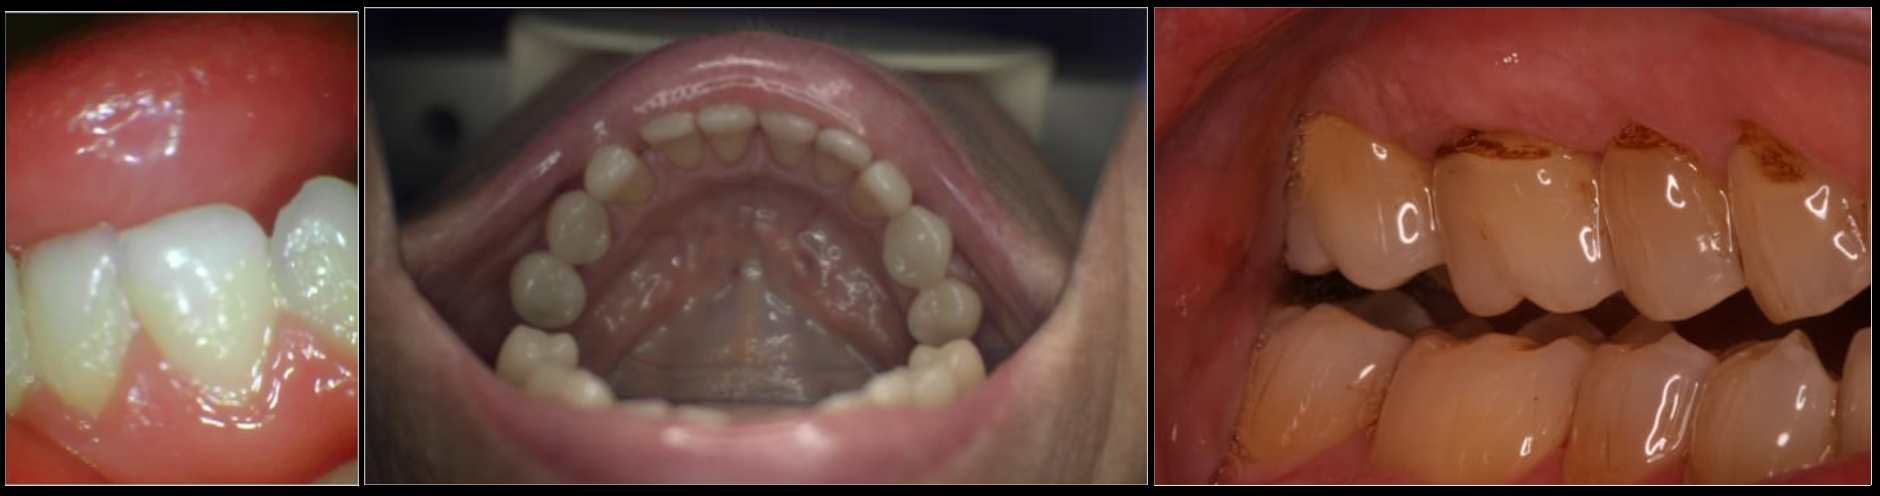
\includegraphics[width=1\textwidth]{recursos/imagens/proposal/image_odonto_dataset.png}
    \label{project:dataset:fig:2}

    Fonte: retirado e adaptado de \cite{You2020, Hyttinen2020} e \textit{Dental Care}, respectivamente.
\end{figure}



\subsection{Experimentos}
\label{project:exp}

- Classificação de Imagens

- Segmentação de Imagens com U-net Like

- Segmentação de Imagens com U-net

\subsection{Avaliação dos Experimentos}
\label{project:exp_result}

